\documentclass[12pt]{article}
\usepackage{geometry}
\usepackage{a4}
\usepackage{amsfonts}
\usepackage{amssymb,amsmath,amsthm}
\usepackage{polski}
\usepackage[utf8]{inputenc}
\usepackage{comment}
\usepackage{braket}
% \usepackage[draft]{graphicx}
\usepackage{graphicx}
\usepackage{verbatim}
\usepackage{framed}
\numberwithin{equation}{section}
\newcommand{\eq}[1]{\begin{equation}#1\end{equation}}
\newcommand{\Der}[2]{\frac{\text{d}#1}{\text{d}#2}}
\theoremstyle{definition}
\usepackage{extarrows,pgffor}
\makeatletter
\renewcommand{\part}[2]{\frac{\partial#1}{\partial#2}}
\usepackage{slashed}
\usepackage{bbold}
\newcommand{\id}{\mathbb{1}}
%\usepackage{cprotect}
\usepackage{float}
\newtheorem*{hyp*}{Hipoteza}
\newtheorem*{defin*}{Definicja}
\usepackage{ragged2e}
\usepackage{extarrows,pgffor}
\usepackage{gnuplottex}
\usepackage{rotating}
\newcommand{\HRule}{\rule{\linewidth}{0.5mm}}

\begin{document}
\begin{titlepage}
\begin{center}

% Upper part of the page. The '~' is needed because \\
% only works if a paragraph has started.

\textsc{\LARGE Instytut Fizyki PAN}\\[1.5cm]

%\textsc{\Large Zakład Optyki Kwantowej}\\[0.5cm]

% Title
\HRule \\[0.4cm]
{ \huge \bfseries „Statystyka ciemnych solitonów w termicznym jednowymiarowym
gazie bozonowym przy pomocy stochastycznego równania
 Grossa-Pitajewskiego” \\[0.4cm] }

\HRule \\[1.5cm]

% Author and supervisor
\noindent
\large Igor Nowicki
\\[2cm]
\begin{flushleft}
Raport z badań przeprowadzonych w ramach projektu\\
\emph{"Procesy spontaniczne w ultrazimnych gazach o niezerowej temperaturze",}\\[1cm]
nr umowy 2012/07/E/ST2/01389 z NCN.\\[2cm]
\end{flushleft}

% {\large \today}

\end{center}
\end{titlepage}

\newcommand{\dx}{\Delta x}
\section{Wstęp}
Badania z tego miesiąca obejmowały zebranie statystyki solitonów dla różnych temperatur i znalezienie korelacji z rozkładem statystycznym modułu funkcji falowej kondensatu Bosego-Einsteina. Przyjmowane parametry układu (w jednostkach własnych):
\begin{align*}
N &= 2048,\\
L &= 204.8,\\
t_\text{total}&=10000,
\end{align*}

gdzie $N$ stanowi liczbę punktów sieci symulowanego układu, $L$ jest jego szerokością, a $t_\text{total}$ to czas ewolucji. W dalszym ciągu symulowane równanie to:

\begin{equation}i\part\psi t=(1-i\gamma)\Big[-\frac12\part{^2}{x^2}-\mu+g|\psi|^2\Big]\phi+\sqrt{\frac{\gamma T}{\Delta x\Delta t}}\times z_0,\end{equation}

gdzie $z_0=s_1+\text is_2$ jest losową liczbą zespoloną, której parametry mają rozkład normalny:

$$\mathcal P(s_i)=\frac1{\sqrt{2\pi}}e^{-s^2_i/2}.$$

Pozostałe parametry mają wartość:

\begin{align*}
\Delta x &= 0.1,\\
\Delta t&=0.01,\\
\gamma &= 0.01,\\
\mu &= 1,\\
g&=0.01.
\end{align*}

\section{Metody zliczania solitonów - porównanie}

Do rozstrzygnięcia pozostaje dobranie odpowiednich parametrów zliczania solitonów w temperaturach $T>100$ jednostek.

\begin{figure}[htbp]
\centering
\begin{gnuplot}[terminal=epslatex,terminaloptions=color]
n="max_val.txt"
plot n u 1:2 t "Max val" w linespoints, n u 1:3 t "Mean value" w linespoints
\end{gnuplot}
\end{figure}

Przedstawię poniżej wyliczone liczby solitonów dla różnych parametrów obcięcia, do porównania z brakiem parametru obcięcia.
% 
% 
% 
% \section{Metoda obcięcia fourierowskiego - modyfikacja}
% 
% Zamierzam zastosować obcięcie nie przez funkcję skoku, a przez funkcję $e^{-x^2/2\sigma^2}$. Poniżej zaprezentuję przykładowe wyniki dla obydwu metod.
% 
% Poniżej przedstawiam mapę uzyskiwanych wyników liczby i grubości solitonów dla różnych progów procentowych średniej wartości $|\Psi|$.
% 
% \begin{figure}[H]
% \centering
% % \begin{minipage}{0.5\linewidth}
% 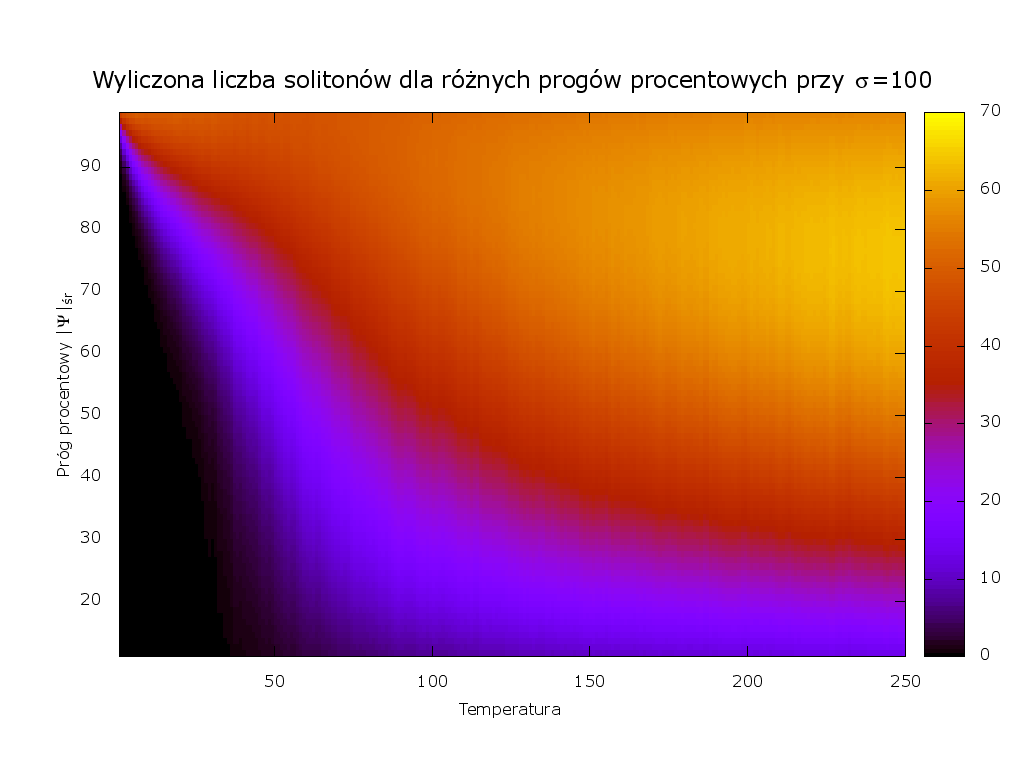
\includegraphics[width=1\linewidth]{percent_a.png}
% % \end{minipage}\begin{minipage}{0.5\linewidth}
% 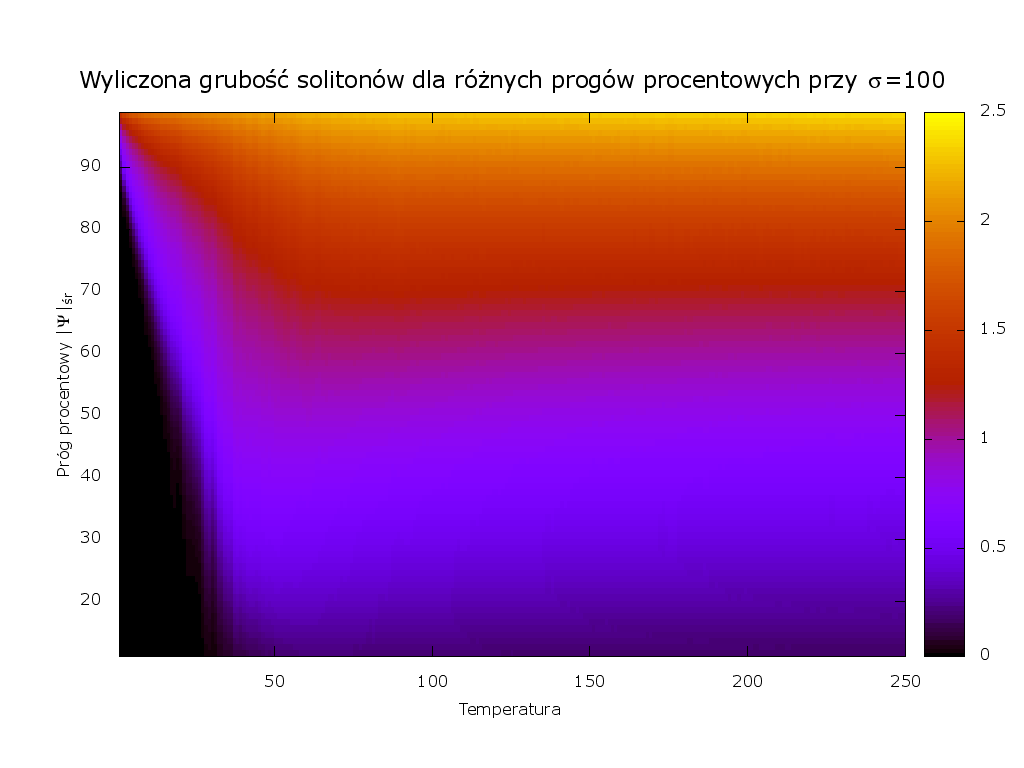
\includegraphics[width=1\linewidth]{percent_b.png}
% % \end{minipage}
% \end{figure}


\end{document} 
